\documentclass{standalone}
\usepackage{pgfplots}
\pgfplotsset{compat=newest}

\begin{document}
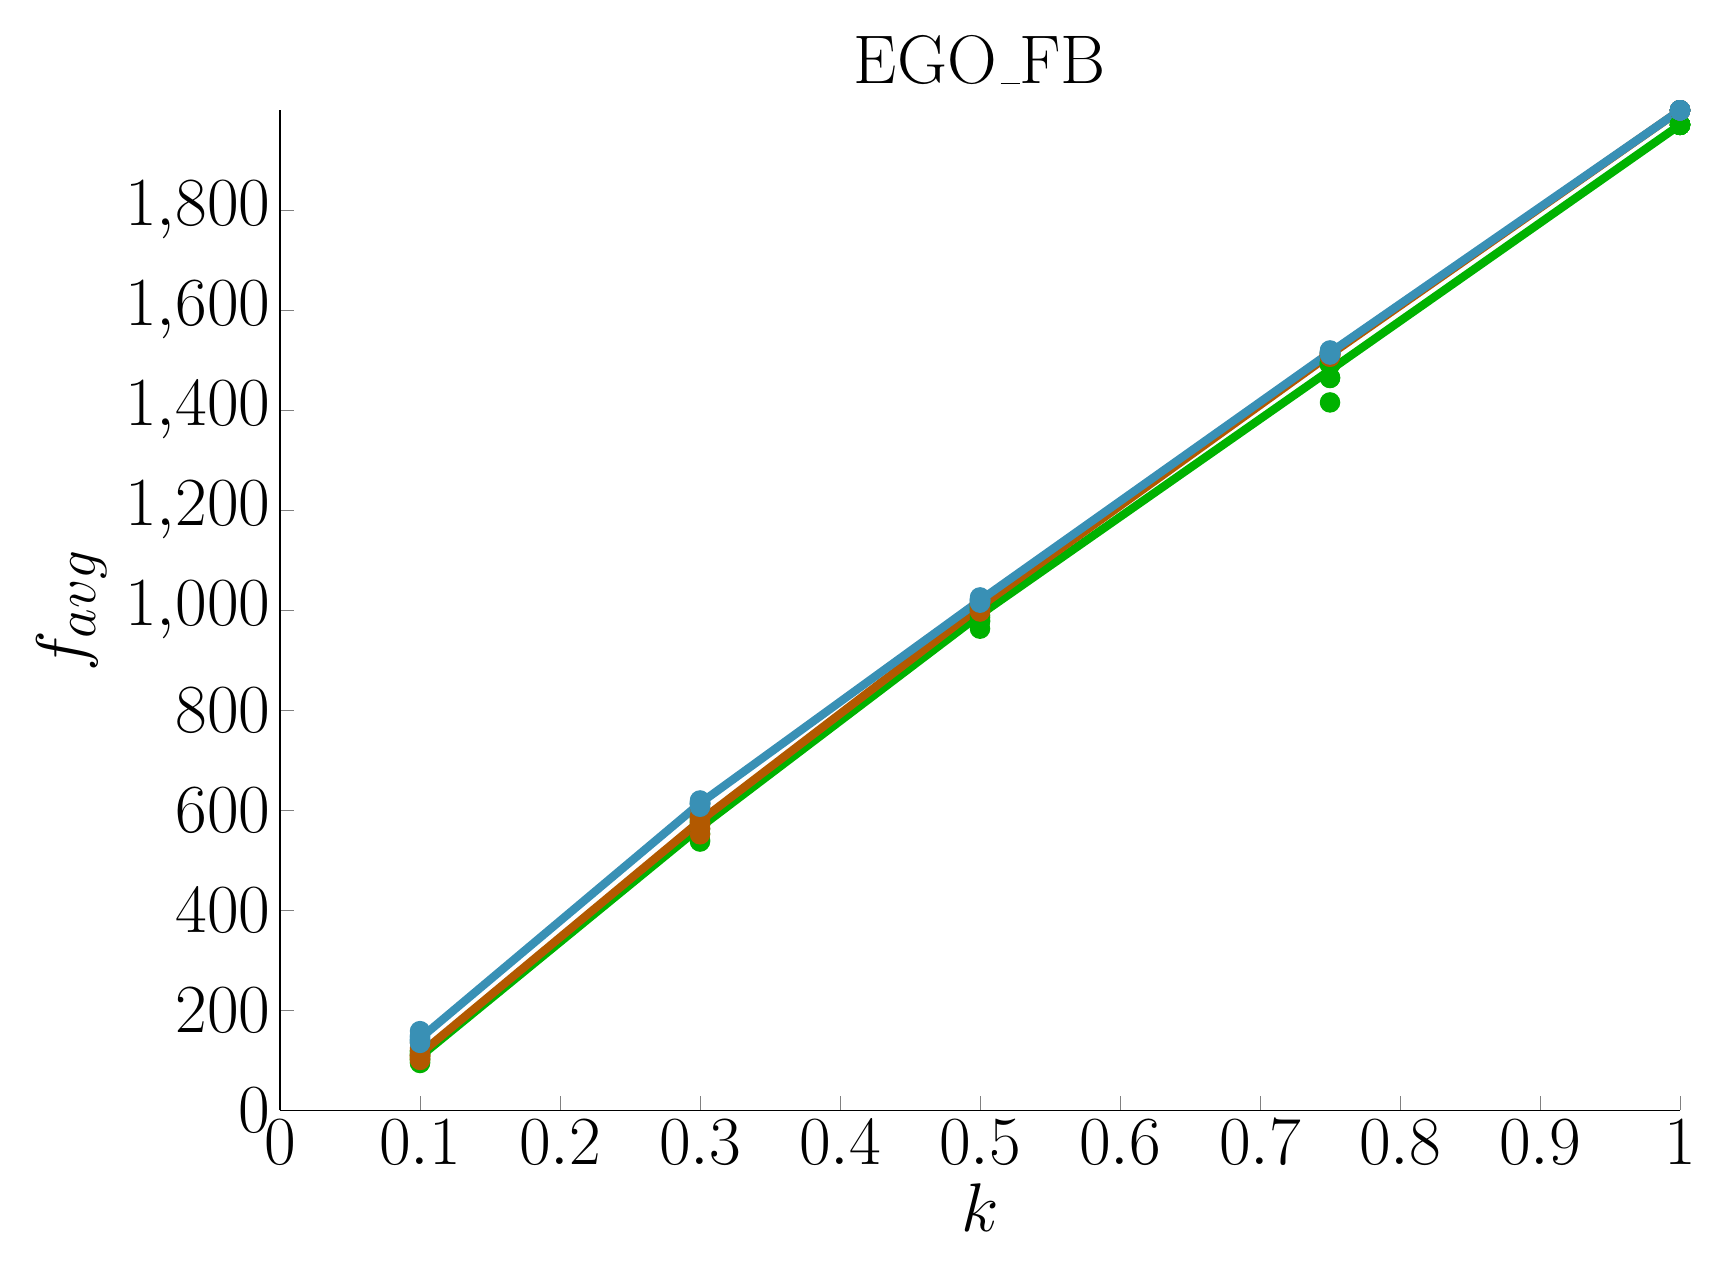
\begin{tikzpicture}

\begin{axis}[%
title style={font=\Huge},
title=EGO\_FB,
tick label style={font=\Huge},
label style={font=\Huge},
legend style={font=\Huge},
view={0}{90},
max space between ticks=50pt,
width=7in,
height=5in,
scale only axis,
xmin=0, xmax=1,
%xtick={0, 20, 40, 60, 80, 100},
xlabel={$k$},
ymin=0, ymax=1999.0,
ylabel={$f_{avg}$},
major tick length=5pt,
axis lines*=left,
legend cell align=left,
clip=false]

\addplot [
only marks,
mark=*,
mark size=3.5pt,
color=green!70!black,
%solid,
%line width=2pt,
]
coordinates{
(0.1,94.58)(0.1,96.26)(0.1,100.44)(0.1,102.64)(0.1,104.4)(0.1,111.04)(0.1,111.16)(0.1,114.38)(0.1,117.76)(0.1,118.42)(0.3,537.22)(0.3,540.22)(0.3,552.72)(0.3,562.4)(0.3,570.78)(0.3,574.24)(0.3,577.34)(0.3,578.04)(0.3,580.14)(0.3,582.12)(0.5,962.78)(0.5,976.48)(0.5,978.96)(0.5,984.74)(0.5,989.78)(0.5,997.08)(0.5,1001.0)(0.5,1002.68)(0.5,1004.86)(0.5,1008.26)(0.75,1415.04)(0.75,1463.84)(0.75,1464.58)(0.75,1490.4)(0.75,1491.96)(0.75,1492.04)(0.75,1492.88)(0.75,1494.84)(0.75,1494.9)(0.75,1495.74)(1,1970.0)(1,1970.0)(1,1970.0)(1,1970.0)(1,1970.0)(1,1970.0)(1,1970.0)(1,1970.0)(1,1970.0)(1,1970.0)
};

\addplot [
only marks,
mark=*,
mark size=3.5pt,
color=orange!70!black,
%solid,
%line width=2pt,
]
coordinates{
(0.1,100.64)(0.1,102.8)(0.1,107.08)(0.1,107.64)(0.1,108.38)(0.1,109.52)(0.1,111.96)(0.1,119.66)(0.1,124.68)(0.1,135.7)(0.3,551.7)(0.3,563.28)(0.3,570.62)(0.3,575.5)(0.3,575.52)(0.3,583.94)(0.3,584.18)(0.3,585.22)(0.3,587.56)(0.3,605.32)(0.5,997.02)(0.5,998.32)(0.5,1000.12)(0.5,1006.12)(0.5,1006.42)(0.5,1009.64)(0.5,1010.48)(0.5,1010.96)(0.5,1013.5)(0.5,1013.92)(0.75,1506.28)(0.75,1506.94)(0.75,1508.96)(0.75,1509.84)(0.75,1510.5)(0.75,1510.54)(0.75,1511.36)(0.75,1511.9)(0.75,1513.58)(0.75,1514.84)(1,1999.0)(1,1999.0)(1,1999.0)(1,1999.0)(1,1999.0)(1,1999.0)(1,1999.0)(1,1999.0)(1,1999.0)(1,1999.0)
};

\addplot [
only marks,
mark=*,
mark size=3.5pt,
color=cyan!70!black,
%solid,
%line width=2pt,
]
coordinates{
(0.1,134.76)(0.1,135.64)(0.1,138.84)(0.1,140.5)(0.1,141.62)(0.1,141.7)(0.1,146.32)(0.1,147.38)(0.1,150.22)(0.1,158.28)(0.3,606.74)(0.3,611.16)(0.3,612.2)(0.3,612.72)(0.3,612.74)(0.3,613.38)(0.3,614.6)(0.3,615.88)(0.3,617.52)(0.3,619.42)(0.5,1014.7)(0.5,1016.12)(0.5,1016.86)(0.5,1017.88)(0.5,1019.12)(0.5,1019.5)(0.5,1020.62)(0.5,1021.52)(0.5,1022.0)(0.5,1025.32)(0.75,1510.7)(0.75,1512.76)(0.75,1513.42)(0.75,1513.78)(0.75,1514.44)(0.75,1514.84)(0.75,1515.02)(0.75,1516.64)(0.75,1517.46)(0.75,1518.98)(1,1999.0)(1,1999.0)(1,1999.0)(1,1999.0)(1,1999.0)(1,1999.0)(1,1999.0)(1,1999.0)(1,1999.0)(1,1999.0)
};
p
\addplot [
color=green!70!black,
solid,
line width=3pt
]
coordinates{
(0.1,107.108)(0.3,565.522)(0.5,990.662)(0.75,1479.622)(1.0,1970.0)
};

\addplot [
color=orange!70!black,
solid,
line width=3pt
]
coordinates{
(0.1,112.806)(0.3,578.284)(0.5,1006.65)(0.75,1510.474)(1.0,1999.0)
};

\addplot [
color=cyan!70!black,
solid,
line width=3pt
]
coordinates{
(0.1,143.526)(0.3,613.636)(0.5,1019.364)(0.75,1514.804)(1.0,1999.0)
};


\end{axis}
\end{tikzpicture}
\end{document}
